\subsection{分别连续双线性映射}

设 E、F、G 是三个局部凸空间。对每个从 \(E \times F\) 到 G 中的双线性映射 u，及每个 \(x \in E\)（相应地，\(y \in F\)），我们用 \(u(x, .)\)（相应地，\(u(., y)\)）记从 F 到 G 中（相应地，从 E 到 G 中）的映射 \(y \mapsto u(x, y)\)（相应地，\(x \mapsto u(x, y)\)）。

定义 1. --- 称从 E × F 到 G 中的双线性映射 u 为分别连续的，如果对所有 x ∈ E，从 F 到 G 中的线性映射 u(x, .) 连续，且对所有 y ∈ F，从 E 到 G 中的线性映射 u(., y) 连续。

下面的命题立即由定义得出。

命题 1. --- 为使从 E × F 到 G 中的双线性映射 u 分别连续，必要且充分的是：对所有 y ∈ F，从 E 到 G 中的线性映射 u(., y) 连续，且从 F 到 \(\mathcal{L}_s(E; G)\) 中的线性映射 y ↦ u(., y) 连续。

我们也可以说，对每个线性映射 \(v \in \mathcal{L}\left(\mathrm{F}; \mathcal{L}_{s}(\mathrm{E}; \mathrm{G})\right)\)，联结双线性映射 \((x, y) \mapsto v(y)(x)\)，于是我们定义了一个从 \(\mathcal{L}(\mathrm{F}; \mathcal{L}_{s}(\mathrm{E}; \mathrm{G}))\) 到从 \(E \times F\) 到 G 中的分别连续双线性映射所成的向量空间上的线性双射。

从 \(E \times F\) 到 G 中的分别连续双线性映射未必在 \(E \times F\) 上连续（III, 第 47 页, 习题 2；但参看 III, 第 30 页 及 IV, 第 26 页, 定理 2）。

两个局部凸空间的乘积 \(E_{1} \times E_{2}\) 上的分别连续双线性型的概念，当 \(E_{1}\) 和 \(E_{2}\) 被赋予弱拓扑时（II, 第 42 页），与连续线性映射的概念直接相关。假设 \((\mathrm{E}_{1}, \mathrm{F}_{1})\) 和 \((\mathrm{E}_{2}, \mathrm{F}_{2})\) 是处于分离对偶中的两对实（相应地，复）向量空间（同前处）；我们给 \(E_{i}\)（相应地，\(F_{i}\)）赋予弱拓扑 \(\sigma(\mathrm{E}_{i}, \mathrm{F}_{i})\)（相应地，\(\sigma(\mathrm{F}_{i}, \mathrm{E}_{i})\)），i = 1, 2，并用 \(\mathrm{B}(\mathrm{E}_{1}, \mathrm{E}_{2})\) 记 \(E_{1} \times E_{2}\) 上的分别连续双线性型所成的向量空间。把命题 1 应用于 G = K 的情形，我们看到，对每个双线性型 \(\Phi \in \mathrm{B}(\mathrm{E}_{1}, \mathrm{E}_{2})\) 和每个 \(x_{2} \in E_{2}\)，映射 \(x_{1} \mapsto \Phi(x_{1}, x_{2})\) 是 \(E_{1}\) 上的一个连续线性型，因而（II, 第 43 页, 命题 3）存在一个且仅一个 \(^{d}\Phi(x_{2}) \in F_{1}\) 使得

\[
\Phi (x _ {1}, x _ {2}) = \langle x _ {1}, ^ {d} \Phi (x _ {2}) \rangle\tag{1}
\]

对所有 \(x_1 \in \mathbf{E}_1\) 和 \(x_2 \in \mathbf{E}_2\) 成立；此外，映射 \(^d\Phi: \mathbf{E}_2 \to \mathbf{F}_1\) 对 \(\mathbf{E}_2\) 和 \(\mathbf{F}_1\) 的（弱）拓扑是线性且连续的。

反之，对每个连续线性映射 \(u: \mathrm{E}_2 \to \mathrm{F}_1\)，映射 \((x_1, x_2) \mapsto \Phi(x_1, x_2) = \langle x_1, u(x_2) \rangle\) 是 \(\mathrm{E}_1 \times \mathrm{E}_2\) 上的一个分别连续双线性型，且我们有 \(u = {}^d\Phi\)。这样我们就定义了一个同构 \(d: \Phi \mapsto {}^d\Phi\)，从 \(\mathrm{B}(\mathrm{E}_1, \mathrm{E}_2)\) 到 \(\mathcal{L}(\mathrm{E}_2; \mathrm{F}_1)\) 上，称为典范的。类似地，公式

\[
\Phi (x _ {1}, x _ {2}) = \langle {} ^ {s} \Phi (x _ {1}), x _ {2} \rangle\tag{2}
\]

定义了一个典范同构 \(s: \Phi \to {}^s\Phi\)，从 \(\mathbf{B}(\mathbf{E}_1, \mathbf{E}_2)\) 到 \(\mathcal{L}(\mathbf{E}_1, \mathbf{F}_2)\) 上；我们显然有交换图

\begin{enumerate}
\def\labelenumi{(\arabic{enumi})}
\setcounter{enumi}{2}
\tightlist
\item
\end{enumerate}

\pandocbounded{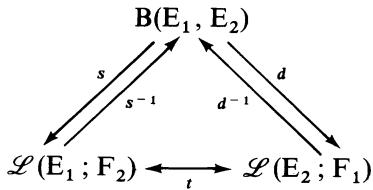
\includegraphics[keepaspectratio]{images/part001_08254dbd.jpg}}

其中 t 是转置同构（II, 第 46 页, 命题 5 及其推论）。鉴于 \(F_{1}\) 和 \(F_{2}\) 上弱拓扑的定义，立即可知：当给 \(\mathbf{B}(\mathbf{E}_{1}, \mathbf{E}_{2})\)、\(\mathcal{L}(\mathbf{E}_{1}; \mathbf{E}_{2})\) 和 \(\mathcal{L}(\mathbf{E}_{2}; \mathbf{F}_{1})\) 赋予简单收敛拓扑时，图 (3) 中的同构都是拓扑向量空间同构。

